The project started at January 21st. From there until February 14th, general plans for the whole project were mapped out, resulting in this preliminary report. The overarching time periods for the different stages in the development of the product and other project work can be seen in the time plan chart below. The first phase of the project emphazises theory, identifying core problems, requirements and possible solutions. It will be an ongoing process throughout the project. 
The second phase, which commences upon the finalization of this report, includes a "rapid prototype" which serves as a base for insights and evaluating theories. This initial prototype will hopefully have working implementations of all importants features of the final prototype and library.  This is the point when the team will start to work as a proper agile team, and three iterations are planned. The deadline for this prototype is set to March 12th, no matter what state the prototype is in at that point.
At the completion of the rapid prototype the actual library will be implemented, and a final prototype will be developed alongside it. At the first week of May, the library should be in a state where it is considered "shippable".The third phase will be ongoing and includes work on the final report which is due on the 19th of May.  

\begin{figure}[h]
\centering
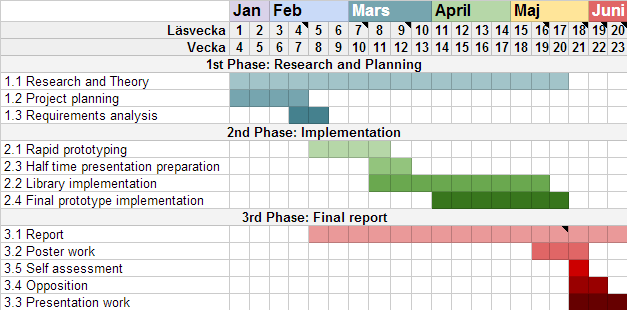
\includegraphics[width=\textwidth,height=0.2\paperheight,keepaspectratio
]{figures/time-plan}
\caption{Time plan for the project}
\label{fig:timeplan}
\end{figure}